\chapter{مفاهیم پایه و تجهیزات‌}

در این فصل به بررسی مفاهیم و تجهیزاتی که در این پروژه استفاده شده‌است می‌پردازیم. در هر بخش دلیل انتخاب خود را شرح می‌دهیم و آن را با سایر راه‌حل‌ها مقایسه می‌کنیم.

\section{حسگر}
همانطور که گفته‌شد برای پیش‌بینی نگهداری و عمر مفید تجهیزات نیاز به نظارت و جمع‌آوری اطلاعاتی راجع‌به این تجهیزات داریم. در این پروژه، اطلاعات جمع‌آوری‌شده مربوط به وضعیت لرزش تجهیزات است که با استفاده از حسگرهای لرزش \lr{MEMS} اندازه‌گیری می‌شوند.


در این پروژه تصمیم گرفتیم که بجای دما یا رطوبت از لرزش تجهیزات برای پیش‌بینی استفاده کنیم؛ زیرا لرزش برخلاف دو معیار دیگر بطور مستقیم شرایط عملیاتی تجهیزات را منعکس می‌کند که بیشتر بر اساس رفتارهای مکانیکی مانند چرخش موتور یا حرکت جریان در لوله ایجاد می‌شوند. هم‌چنین دو معیار دیگر وابستگی زیادی به محیط دارند اما لرزش تقریبا مستقل از عوامل خارجی است\cite{jung2017vibration}.


برای اندازه‌گیری لرزش دو نوع حسگر لرزش وجود دارد. حسگرهای مبتنی بر شتاب‌سنج \lr{MEMS} بر اکثر محدودیت‌های حسگرهای قدیمی مبتنی بر شتاب‌سنج پیزوالکتریک\LTRfootnote{Piezoelectric} غلبه می‌کنند. تفاوت این دو حسگر را می‌توان در \cref{sensor_comparison} \cite{jung2017vibration} دید.

\begin{table}[h!]
  \begin{center}
    \caption{مقایسه بین دو نوع حسگر مبتنی بر پیزوالکتریک و \lr{MEMS} \cite{jung2017vibration}}
    \label{sensor_comparison}
    \begin{tabular}{|c|c|c|} % <-- Alignments: 1st column left, 2nd middle and 3rd right, with vertical lines in between
    \hline
    	& پیزوالکتریک & \lr{MEMS}\\
    	\hline
    	قیمت (دلار) & +۳۰۰ & +۱۰\\
    	\hline
    	توان مصرفی ($mW$) & ۲۷ & ۳\\
    	\hline
    	اندازه (اینچ) & ۱/۹۷ × ۰/۹۸ × ۱ & ۰/۲ × ۰/۲ × ۰/۰۵\\
    	\hline
    	تراکم نویز ($\mu g$) & ۷۰۰ & ۴۰۰۰\\
    	\hline
    	بازه شتاب ($g$) & ۱۰ & ۱۰۰\\
    	\hline
    \end{tabular}
  \end{center}
\end{table}

بطور کلی حسگرهای نوع \lr{MEMS} ارزان‌تر، کم‌مصرف‌تر و کوچک‌تر هستند. در این پروژه حسگرها با باتری کار خواهند کرد و برای اندازه‌گیری به قطعات مورد نظر متصل می‌شوند. بنابراین کم‌مصرف‌بودن، ارزانی و کوچک‌بودن برای اتصال به بدنه ویژگی‌های مطلوبی است که در حسگرهای نوع \lr{MEMS} یافت می‌شود. \cref{fig:sensor} حسگر مدل \lr{ADXL 345} که در این پروژه استفاده کرده‌ایم.

\begin{figure}[!h]
\centering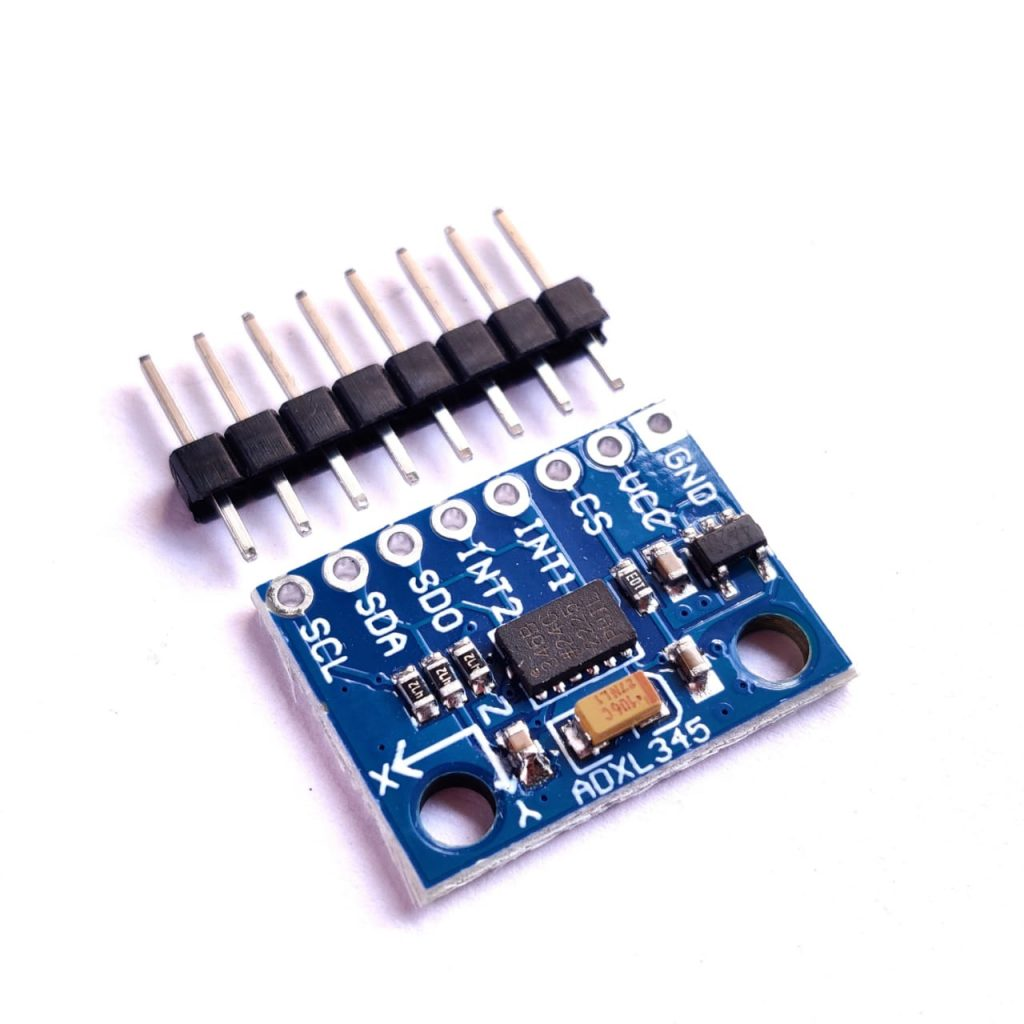
\includegraphics[scale=0.15]{sensor.png}
\caption{حسگر مدل \lr{ADXL 345}}\label{fig:sensor}
\end{figure}

این حسگر می‌تواند شتاب را در سه جهت، در چهار بازه قابل تنظیم ۲، ۴، ۸ و ۱۶ برابر گرانش با دقت‌های متفاوت اندازه‌گیری کند. خروجی این حسگر نیز با دو پروتکل \lr{SPI}\LTRfootnote{Serial Peripheral Interface} و \lr{I2C} قابل انتقال است.

\section{گره انتهایی}

برای کاهش بیشتر مصرف انرژی، دریافت اطلاعات حسگر و فرستادن آن برای دروازه به یک بورد\LTRfootnote{Board} نیاز داریم. بوردهای آردوینو\LTRfootnote{Arduino} اگرچه محدودیت‌هایی دارند، اما با توجه به ارزان‌بودن و برآورده‌کردن نیاز ما انتخاب مناسبی هستند. بورد استفاده‌شده در این پروژه آردوینو نانو است که در \cref{fig:arduino_nano} قابل‌مشاهده است. در این بورد از پورت سریال\LTRfootnote{Serial Port} برای ارتباط با ماژول زیگبی\LTRfootnote{Zigbee Module} و از پروتکل \lr{I2C} برای ارتباط با حسگر استفاده می‌کنیم. یکی از محدودیت‌های این بورد حافظه کم است که در نرخ‌های بالای نمونه‌برداری حسگر کار ما را سخت می‌کند که در فصل بعد بیشتر به آن می‌پردازیم.

\begin{figure}[!h]
\centering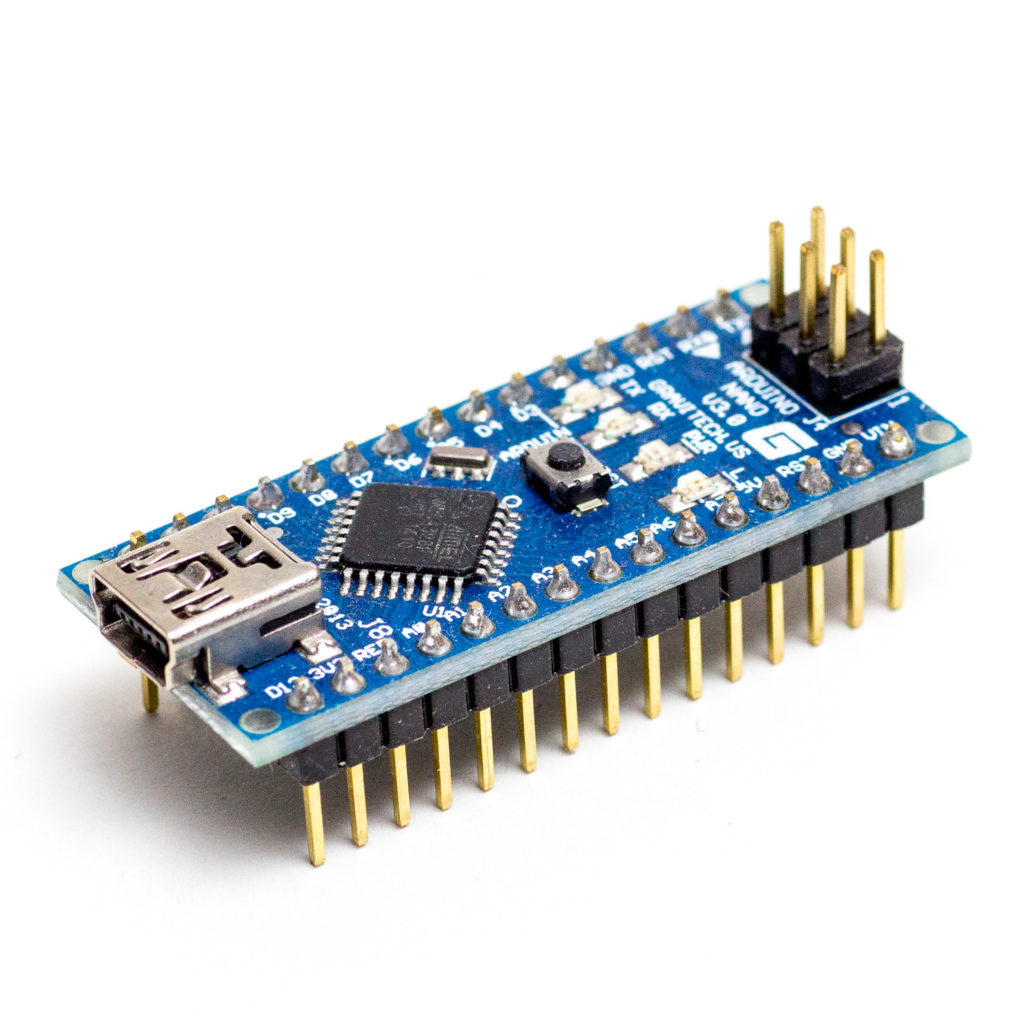
\includegraphics[scale=0.15]{arduino_nano.png}
\caption{بورد آردوینو نانو}\label{fig:arduino_nano}
\end{figure}

\section{پروتکل ارتباطی}

برای ارسال اطلاعات از گره‌های متصل به حسگر به دروازه نیاز به یک پروتکل ارتباطی داریم. نیازهای ما در رابطه با این پروتکل عبارتند از:
\begin{itemize}
\item کم‌مصرف‌بودن: با توجه به اینکه گره‌های ما به باتری متصل هستند، به پروتکلی نیاز داریم که در مصرف انرژی بسیار بهینه عمل کند تا بتوان بدون تعویض باتری اطلاعات را تا چند سال برای دروازه فرستاد.
\item پوشش و نفوذ سیگنال: در هر کارخانه یک دروازه نصب شده‌است، کارخانه‌ها مساحتی متوسط دارند و مانع خاصی نیز در آنها وجود ندارد. پس نیاز به پوشش یا قدرت نفوذ بالایی در سیگنال ارسالی نداریم.
\item توپولوژی\LTRfootnote{Topology}: با توجه به وجود یک دروازه و چندین گره که همگی اطلاعات را برای دروازه ارسال می‌کنند، نیاز به پروتکلی داریم که از توپولوژی ستاره پشتیبانی کند.
\item ارتباط مطمئن\LTRfootnote{Reliable Communication}: ارسال ناقص و یا از دست‌دادن اطلاعات حسگرها می‌تواند باعث پیش‌بینی اشتباه شود. بنابراین، به پروتکلی با قابلیت ارتباط مطمئن و کنترل خطا نیاز داریم.
\end{itemize}

در \cref{fig:protocol_comp} پروتکل‌های ارتباطی با معیارهای مختلف مقایسه شده‌اند. بر اساس ویژگی‌های موردنیاز پروتکل زیگبی انتخاب مناسب‌تری نسبت به سایر پروتکل‌ها است که در ادامه آن را معرفی می‌کنیم.

\begin{figure}
\centering
\begin{subfigure}{.5\textwidth}
  \centering
  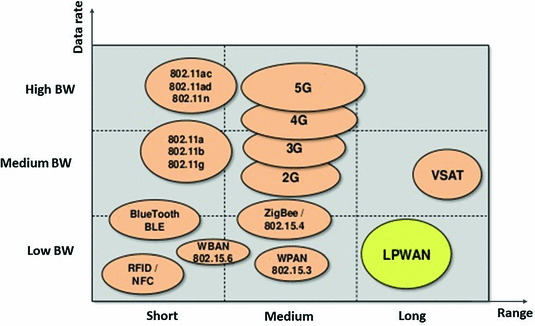
\includegraphics[height=5cm, width=.9\linewidth]{protocol_data_range.png}
    \centering
  \caption{مقایسه بر حسب نرخ داده و بازه پوشش \cite{carlsson2018measuring}}
\end{subfigure}%
\begin{subfigure}{.5\textwidth}
  \centering
  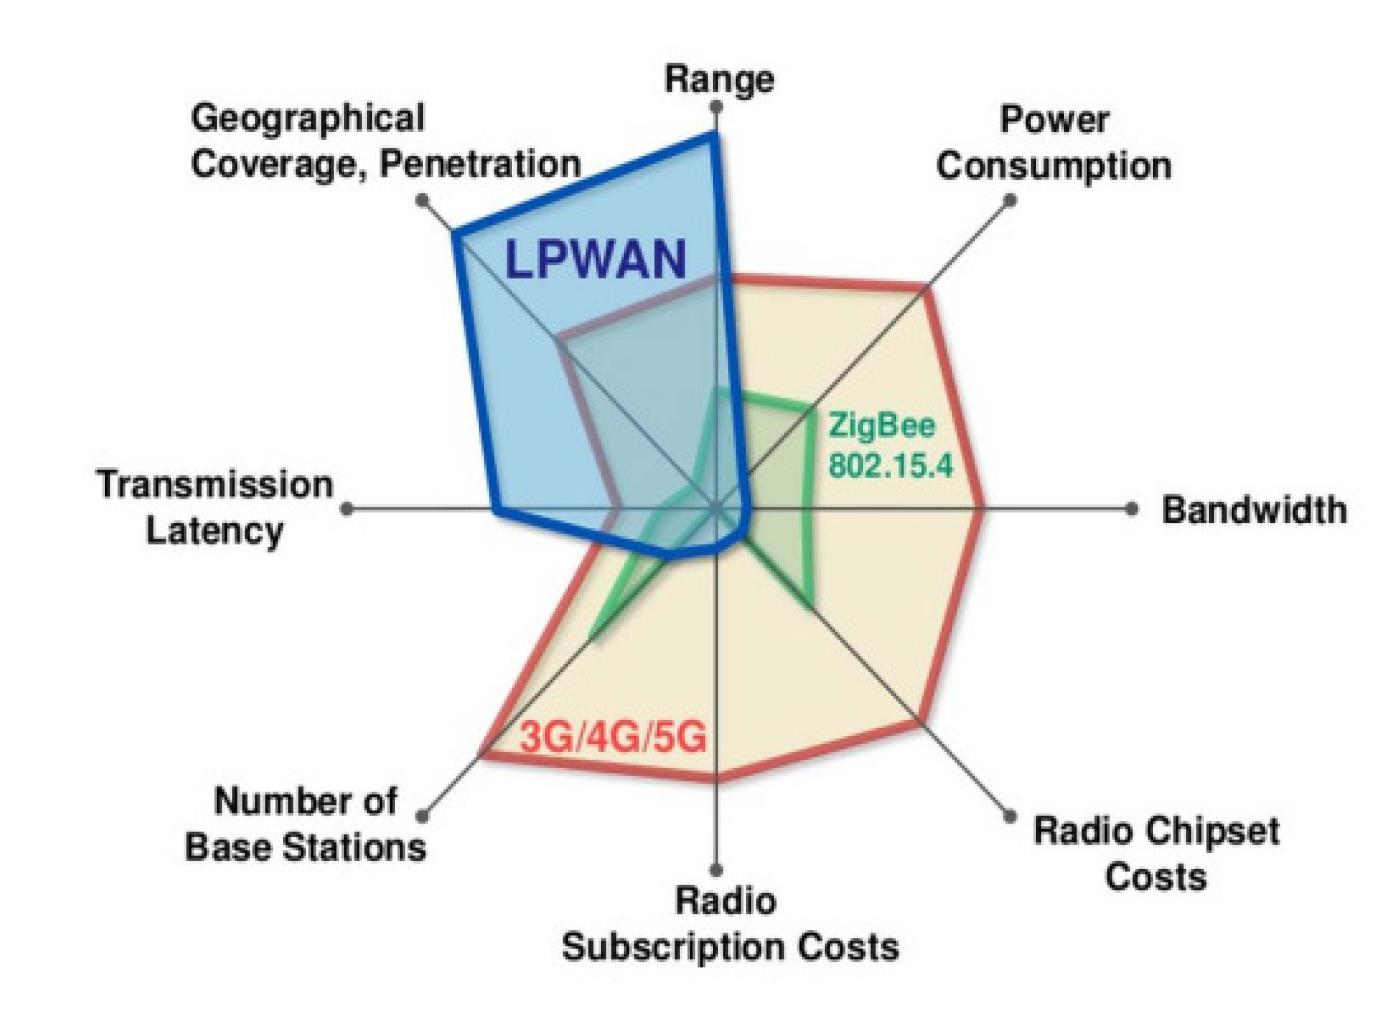
\includegraphics[height=5cm, width=.9\linewidth]{protocol_m_criteria.png}
    \centering
  \caption{مقایسه بر حسب انرژی، بازه پوشش، نفو‌ذ، تاخیر، هزینه و پهنای باند \cite{tabbane2017iot}}
\end{subfigure}
\caption{مقایسه پروتکل زیگبی و سایر پروتکل‌های اینترنت اشیاء}
\label{fig:protocol_comp}
\end{figure}

\subsection{استاندارد زیگبی}

زیگبی یکی از استانداردهای فرستنده-گیرنده\LTRfootnote{Tranceiver} در شبکه‌های حسگر بی‌سیم\LTRfootnote{Wireless Sensor Network} است که بصورت گسترده مورد استفاده قرار گرفته‌است. زیگبی بر روی \lr{IEEE802.15.4} مشخصات شبکه شخصی بی‌سیم با نرخ داده پایین\LTRfootnote{Low Rate Wireless Personal Area Network(LR-WPAN} را تعریف می‌کند تا بتواند از دستگاه‌های نظارتی و کنترلی با توان مصرفی و نرخ داده پایین پشتیبانی کند. زیگبی توسط اتحاد زیگبی\LTRfootnote{Zigbee Alliance} توسعه داده شده‌است؛ که صدها عضو دارد. اتحاد زیگبی لایه‌های شبکه، امنیت و برنامه و \lr{IEEE802.15.4} لایه‌های سخت‌افزار و کنترل دسترسی به رسانه\LTRfootnote{Media Access Control(MAC)} را تعریف می‌کنند\cite{ramya2011study}.

استاندارد شبکه بی‌سیم زیگبی جای خالی‌ای را در بازار پر می‌کند که توسط سایر شرکت‌ها نادیده گرفته شده‌است. 
اکثر استانداردهای بی‌سیم به دنبال نزدیک‌شدن به اینترنت و رسیدن به سرعت‌های بالاتر هستند. اما زیگبی در تلاش است تا با ارائه نرخ ارسال پایین‌تر انتظار مصرف انرژی پایین را برآورده کند. سایر استانداردها به دنبال افزودن ویژگی\LTRfootnote{Feature}های بیشتر و ارائه خدماتی نظیر استریم با کیفیت بالا\LTRfootnote{High-Definition Streaming} هستند؛ درحالیکه زیگبی با پشته\LTRfootnote{Stack}‌ای کوچک تنها هدف دارد که بتوان داده‌هایی با حجم کم و تعدد پایین مانند کنترل چراغ یا خواندن داده‌های سنسور دما را ارسال کرد\cite{gislason2008zigbee}.

\subsection{ویژگی‌های زیگبی}

\subsubsection{قابلیت اطمینان بالا}

ارتباطات بی‌سیم بطور کلی ارتباطات نامطمئنی هستند اما زیگبی در چند سطح قابلیت اطمینان بالایی فراهم می کند که عبارتند از:

\begin{itemize}
\item \lr{IEEE802.15.4}: در آن از ترکیبی از فناوری‌هایی مانند \lr{O-QPSK}\LTRfootnote{Offset-Quadrature Phase-Shift Keying} و \lr{DSSS}\LTRfootnote{Direct Sequence Spread Spectrum} استفاده می‌شود که کارایی بسیار خوبی در محیط‌های با نرخ سیگنال به نویز پایین دارند\cite{gislason2008zigbee}.
\item \lr{CSMA-CA}\LTRfootnote{Carrier Sense Multiple Access Collision Avoidance}: زیگبی از این فناوری برای کنترل دسترسی به رسانه استفاده می‌کند. قبل از ارسال زیگبی به کانال گوش می‌دهد. اگر کسی در حال ارسال نباشد، اطلاعات خود را ارسال می‌کند. این روند از تداخل اطلاعات فرستنده‌های محتلف و ایجاد نیاز برای ارسال دوباره جلوگیری می‌کند\cite{gislason2008zigbee}.
\item کنترل خطا: در هر فریم\LTRfootnote{Frame} زیگبی از \lr{CRC}\LTRfootnote{Cyclic Redundancy Check} ۱۶ بیتی بعنوان چک‌سام\LTRfootnote{Checksum} استفاده می‌شود که قابلیت تشخیص خطا در هر فریم را ایجاد می‌کند\cite{gislason2008zigbee}.
\item فریم تایید: هر فریم در کل ۴ بار برای مقصد ارسال می‌شود(۳ بار ارسال مجدد). اگر باز هم فریم نتواند ارسال شود به مبدا اطلاع داده می‌شود\cite{gislason2008zigbee}.
\end{itemize}

\subsubsection{مصرف انرژی پایین}

ماژول‌های زیگبی در مصرف انرژی بسیار بهینه هستند. یک شبکه زیگبی می‌تواند تا چند سال تنها با استفاده از باتری عمل کند. اگر استفاده از زیگبی به‌درستی مدیریت شود این زمان حتی می‌تواند به عمر باتری اگر بدون استفاده در قفسه بماند برسد. دلیل این استفاده کم این است که گره‌های زیگبی می‌توانند به خواب بروند. نیازی به نگه‌داشتن ارتباط برای باقی‌ماندن در شبکه ندارند\cite{gislason2008zigbee}.

\subsubsection{امنیت بالا}

زیگبی با استفاده از استاندارد رمزگذاری پیشرفته\LTRfootnote{Advanced Encryption Standard(AES)} باعث می‌شود که تنها فرستنده و گیرنده از محتویات فریم اطلاع داشته باشند. هم‌چنین روندی برای احراز هویت گره‌ها هنگام اضافه‌شدن به شبکه بکار می‌برد که مانع اضافه‌شدن گره‌های مخرب به شبکه می‌شود\cite{gislason2008zigbee}.

\subsection{دسته‌بندی دستگاه‌ها}

\subsubsection{دسته‌بندی فیزیکی}
با توجه به توانایی‌های پردازشی دو نوع دستگاه در \lr{IEEE802.15.4} آورده شده‌است:

\begin{itemize}
\item دستگاه با عملکرد کامل\LTRfootnote{Fully Functional Device(FFD)}: این دستگاه‌ها توانایی انجام همه‌ی اعمال استاندارد مانند مسیریابی\LTRfootnote{Routing}، هماهنگی\LTRfootnote{Coordination} و ارسال اطلاعات حسگر را دارند. در استاندارد فعلی این دستگاه‌ها باید همیشه روشن باشند\cite{ramya2011study}.
\item دستگاه با عملکرد کاهش‌یافته\LTRfootnote{Reduced Functional Device(RFD)}: این دستگاه‌ها تنها توانایی ارسال داده‌های حسگر را دارند و مي‌توانند به خواب بروند\cite{ramya2011study}.
\end{itemize}

\subsubsection{دسته‌بندی منطقی}

در این دسته‌بندی سه نوع دستگاه وچود دارد:
\begin{itemize}
\item هماهنگ‌کننده: ریشه درخت شبکه را تشکیل می دهد و می‌تواند به شبکه‌های دیگر متصل شود. در هر شبکه دقیقا یک هماهنگ‌کننده وجود دارد. هماهنگ‌کننده مسئول راه‌اندازی شبکه و انتخاب پارامترهای شبکه مانند کانال فرکانس رادیویی\LTRfootnote{Radio Frequency Channel}، شناسه یکتای شبکه و تنظیم سایر پارامترهای عملیاتی است. همچنین می‌تواند اطلاعات مربوط به شبکه و کلیدهای امنیتی را ذخیره کند\cite{ramya2011study}.
\item مسیریاب: مسیریاب بعنوان گره‌ میانی عمل می‌کند و داده‌ها را از دستگاه‌های دیگر منتقل می‌کند. مسیریاب می‌تواند به یک شبکه از قبل موجود متصل شود، همچنین می‌تواند درخواسات اتصال سایر دستگاه‌ها را بپذیرد و نوعی فرستنده مجدد به شبکه باشد\cite{ramya2011study}.
\item گره پایانی: این دستگاه می‌تواند دستگاه‌های کم‌مصرف یا با باتری باشد. آنها می‌توانند اطلاعات مختلفی را از حسگرها جمع‌آوری کنند و عملکرد کافی برای صحبت با والدین خود(هماهنگ‌کننده یا مسیریاب) را دارند اما نمی‌توانند داده‌ها را از دستگاه‌های دیگر ارسال کنند. این عملکرد کاهش‌یافته امکان کاهش هزینه را فراهم می‌کند. این دستگاه‌ها مجبور نیستند تمام مدت بیدار بمانند، درحالیکه دستگاه‌های متعلق به دو دسته دیگر باید بیدار بمانند\cite{ramya2011study}. 
\end{itemize}

در \cref{fig:zigbee_network} \cite{song2019research} می‌توان یک شبکه زیگبی را که شامل یک هماهنگ‌کننده، چند مسیریاب و چند گره پایانی است را مشاهده کرد.

\begin{figure}[!h]
\centering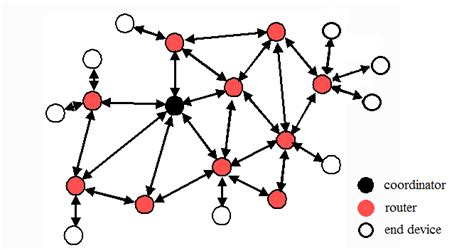
\includegraphics[scale=1]{zigbee_network.png}
\caption{شبکه زیگبی شامل هماهنگ‌کننده، مسیریاب و گره‌پایانی \cite{song2019research}}\label{fig:zigbee_network}
\end{figure}

\subsection{توپولوژی}

در زیگبی می‌توان سه توپولوژی زیر را داشت:

\begin{itemize}
\item ستاره: توپولوژی ستاره از یک هماهنگ کننده و تعدادی دستگاه پایانی تشکیل شده‌است. در توپولوژی ستاره، یک مدل شبکه \lr{master slave} اتخاذ می شود که در آن \lr{master} هماهنگ‌کننده و دستگاهی با عملکرد کامل است و \lr{slave} دستگاهی با عملکرد کامل یا کاهش‌یافته است. دستگاه‌های انتهایی  زیگبی بصورت فیزیکی و الکتریکی از یکدیگر جدا می‌شوند و اطلاعات را تنها از طریق هماهنگ‌کننده منتقل می‌کنند\cite{ramya2011study}.
\item درخت خوشه‌ای\LTRfootnote{Cluster Tree}: این توپولوژی مانند توپولوژی ستاره است، با ابن تفاوت که در این توپولوژی سایر دستگاه‌ها می‌توانند با یکدیگر ارتباط برقرار کنند تا دستگاه‌های بیشتری بتوانند به دستگاه‌های با عملکرد کامل و غیر هماهنگ‌کننده متصل شوند تا بتوان شبکه را از لحاظ جغرافیایی گسترش داد\cite{ramya2011study}.
\item مش\LTRfootnote{Mesh}: در توپولوژی مش، هر گره می‌تواند با هر گره دیگری در محدوده‌ی خود ارتباط برقرار کند. توپولوژی مش برای نگهداری پیچیده است اما نسبت به خطا مقاوم‌تر و قابل‌تحمل‌تر است\cite{ramya2011study}.

در \cref{fig:zigbee_topology} \cite{salih2012design} می‌توان نقش گره‌های مختلف در توپولوژی‌های ذکرشده را مشاهده کرد.

\begin{figure}[!h]
\centering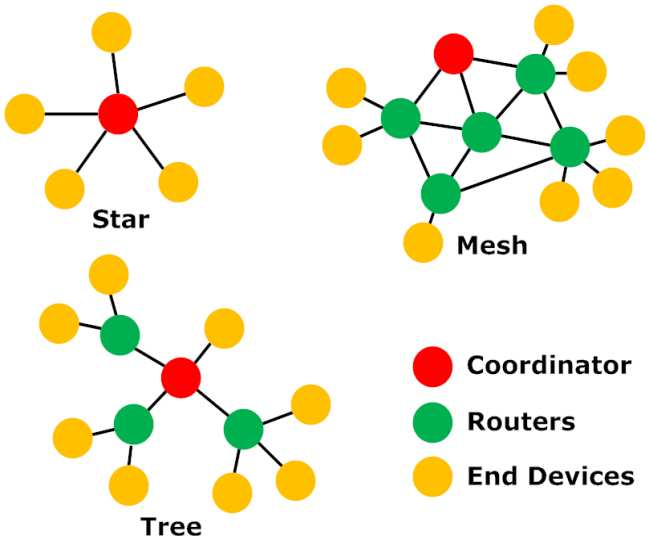
\includegraphics[scale=.4]{zigbee_topology.png}
\caption{توپولوژی‌های مختلف شبکه زیگبی \cite{salih2012design}}\label{fig:zigbee_topology}
\end{figure}
\end{itemize}

\subsection{دیجی بین‌الملل}

دیجی بین‌الملل\LTRfootnote{Digi International} نام یکی از تولیدکنندگان ماژول‌های زیگبی است. ماژولی که ما در این پروژه استفاده می‌کنیم تولید این شرکت است. مدل این ماژول \lr{Digi XBee S2} است که ‌می‌توان تصویر آن را در \cref{fig:XBee_module} مشاهده کرد.

\begin{figure}[!h]
\centering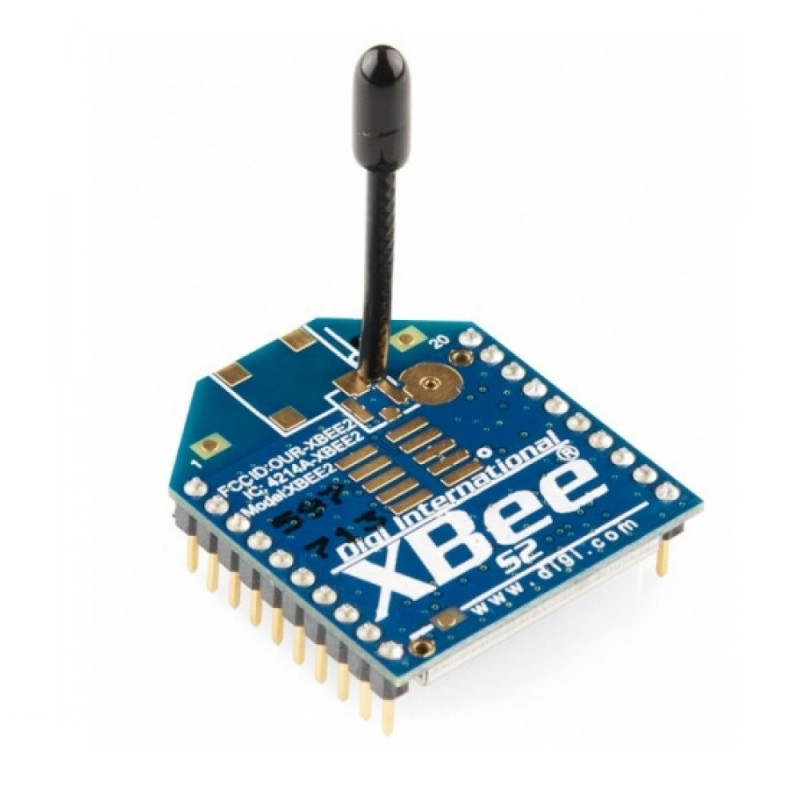
\includegraphics[scale=.25]{XBee_module.png}
\caption{ماژول زیگبی مدل \lr{XBee S2}}\label{fig:XBee_module}
\end{figure}
\end{itemize}

\subsection{طرز کار دستگاه‌های ایکس‌بی}

دستگاه‌های ایکس‌بی از طریق هوا با یکدیگر ارتباط برقرار می‌کنند و پیام‌ها را به‌شکل بی‌سیم ارسال و دریافت می‌کنند. دستگاه‌ها فقط می‌توانند پیام‌ها را منتفل کنند ولی نمی‌توانند آنها را مدیریت کنند. با این‌حال، ماژول‌ها می‌توانند با دستگاه‌های هوشمند از طریق رابط سریال ارتباط برقرار کنند.


دستگاه‌های ایکس‌بی داده‌های ورودی سریال را از طریق هوا منتقل می‌کنند و هر چیزی را که بصورت بی‌سیم دریافت می‌شود به خروجی سریال می‌فرستند. چه برای مقاصد ارتباطی و چه صرفاً برای پیکربندی دستگاه، ترکیبی از هر دو فرایند برای برقراری ارتباط لازم است. به این صورت، دستگاه‌های هوشمند مانند میکروکنترلر\LTRfootnote{Microcontroller}ها یا رایانه‌های شخصی می‌توانند آنچه را که دستگاه ارسال می‌کند کنترل کرده و پیام‌های دریافتی و ارسالی را مدیریت کنند\cite{Digi}.

دو فرایند لازم برای ارتباط را می‌توان در \cref{fig:xbee_communication} \cite{Digi} دید که عبارتند از:
\begin{itemize}
\item ارتباط بی‌سیم: این ارتباط بین ماژول‌های ایکس‌بی انجام می‌شود. ماژول‌هایی که قرار است با هم کار کنند باید بخشی از یک شبکه باشند و باید از یک فرکانس رادیویی استفاده کنند. همه ماژول‌هایی که این الزامات را برآورده می‌کنند می‌توانند بصورت بی‌سیم با یکدیگر ارتباط برقرار کنند.
\item ارتباط سریال: این ارتباط بین ماژول ایکس‌بی و دستگاه هوشمند متصل به آن از طریق رابط سریال صورت می‌گیرد.
\end{itemize}

\begin{figure}[!h]
\centering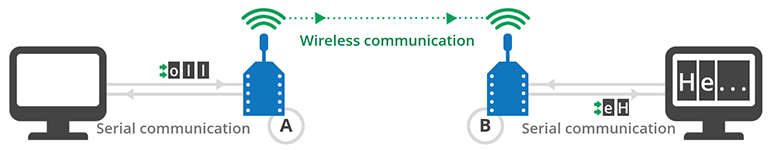
\includegraphics[scale=.7]{xbee_communication.png}
\caption{فرایندهای لازم برای ارتباط دو ماژول ایکس‌بی \cite{Digi}}\label{fig:xbee_communication}
\end{figure}

\subsection{ارتباط سریال ماژول‌های ایکس‌بی}

دستگاه‌های ایکس‌بی می‌توانند از اتصال سریال محلی خود به روش‌های بسیار متفاوتی استفاده کنند. حالت عملیاتی نحوه ارتباط دستگاه میزبان با ماژول ایکس‌بی را از طریق رابط سریال تعیین می‌کند. این حالت‌ها به دو دسته تقسیم می‌شوند که در ادامه به شرح هر کدام می‌پردازیم.

\subsubsection{حالت شفاف}

هنگام کار در حالت شفاف\LTRfootnote{Transparent Mode}، یک ماژول ایکس‌بی بعنوان جایگزین خط سریال عمل می‌کند. تمام داده‌های دریافت‌شده از طریق ورودی سریال بلافاصله از طریق هوا منتقل می‌شود. هنگامی که ماژول ایکس‌بی داده‌های بی‌سیم را دریافت می‌کند، از طریق رابط سریال به همان شکل محل دریافت‌شده ارسال می‌شود. در واقع، ارتباط در حالت شفاف مانند آن است که دو ماژول توسط یک سیم به هم متصل شده‌باشند\cite{Digi}.


برای ارتباط دو ماژول ایکس‌بی، ماژول ارسال‌کننده به آدرس گیرنده نیاز دارد. هنگام کار در حالت شفاف، باید این آدرس را در ماژولی که در حال ارتباط است پیکربندی کرد. ماژول‌های ایکس‌بی می‌توانند آدرس ۶۴ بیتی کامل ماژول مقصد را ذخیره کنند\cite{Digi}. این آدرس باید در دو پارامتر نوشته شود: آدرس مقصد بالا\LTRfootnote{Destination Address High(DH)} و آدرس مقصد پایین\LTRfootnote{Destination Address Low(DL)}. بعنوان مثال برای ارتباط دو ماژول در این حالت باید مثل \cref{fig:transparent_config} \cite{Digi} دو ماژول را پیکربندی کرد.


\begin{figure}[!h]
\centering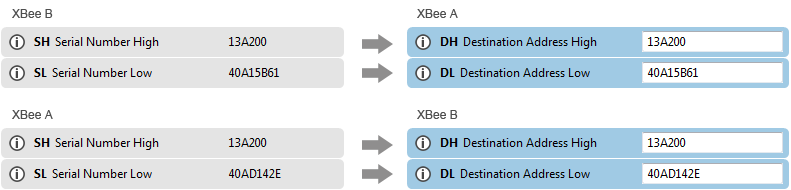
\includegraphics[scale=.7]{transparent_config.png}
\caption{ارتباط سریال در حالت شفاف \cite{Digi}}\label{fig:transparent_config}
\end{figure}

حالت شفاف محدودیت‌هایی دارد. بعنوان مثال، هنگام کار با چند ماژول، باید قبل از ارسال هر پیام، مقصد را پیکربندی کرد. با این حال، حالت شفاف به دلایل زیر راهی آسان برای شروع کار با دستگاه‌های ایکس‌بی فراهم می‌کند:

\begin{itemize}
\item عملیات بسیار ساده است.
\item آنچه ارسال می‌شود دقیقا همان چیزی است که در ماژول دیگر دریافت می‌شود.
\item سازگار با هر دستگاهی است که بتواند از طریق یک رابط سریال ارتباط برقرار کند.
\end{itemize}

\subsubsection{حالت \lr{API}}

حالت \lr{API} یک رابط ساختاریافته را فراهم می‌کند که در آن داده‌ها از طریق رابط سریال در بسته‌های سازماندهی‌شده و به ترتیب تعیین‌شده ارتباط برقرار می‌کنند. این روند اجازه می‌دهد بدون نیاز به تعریف پروتکل، ارتباط پیچیده بین دستگاه‌ها برقرار کرد\cite{Digi}.

در حالت شفاف تمام داده‌های دریافت‌شده از طریق ورودی سریال برای ارسال رادیویی در صف قرار می‌گیرند و داده‌های دریافت‌شده به‌صورت بی‌سیم دقیقاً همان‌طور که دریافت شده‌اند، بدون اطلاعات اضافی به خروجی سریال ارسال می‌شوند\cite{Digi}.

به دلیل این رفتار، دستگاه‌هایی که در حالت شفاف کار می‌کنند محدودیت‌هایی دارند:
\begin{itemize}
\item برای خواندن یا نوشتن پیکربندی یک دستگاه در حالت شفاف، ابتدا باید دستگاه را به حالت فرمان تغییر داد.
\item اگر دستگاهی نیاز به انتقال پیام به دستگاه‌های مختلف داشته‌باشد، باید پیکربندی آن برای ایجاد یک مقصد جدید بروز شود. دستگاه باید برای تنظیم مقصد وارد حالت فرمان شود.
\item دستگاهی که در حالت شفاف کار می‌کند نمی‌تواند منبع پیام بی‌سیمی را که دریافت کرده شناسایی کند. اگر نیاز به تمایز بین داده‌های دریافتی از دستگاه‌های مختلف باشد، دستگاه‌های فرستنده باید شامل اطلاعات اضافی شناخته‌شده توسط همه دستگاه‌ها باشند تا بتوان بعداً آنها را استخراج کرد.
\end{itemize}

حالت \lr{API} راه بسیار آسان‌تری برای انجام اقدامات ذکرشده ارائه می‌دهد:

\begin{itemize}
\item از آنجایی که فریم‌های مختلفی برای اهداف مختلف (مانند پیکربندی و ارتباط) وجود دارد، می‌توان یک دستگاه را بدون وارد شدن به حالت فرمان پیکربندی کرد.
\item از آنجایی که مقصد داده بعنوان بخشی از ساختار فریم \lr{API} گنجانده شده‌است، می‌توان از حالت \lr{API} برای انتقال پیام‌ها به چندین دستگاه استفاده کرد. 
\item فریم \lr{API} همانطور که در \cref{fig:api_mode} \cite{Digi} نشان داده شده‌است، شامل منبع پیام است. بنابراین تشخیص اینکه داده‌ها از کجا آمده‌اند آسان است.
\end{itemize}

\begin{figure}[!h]
\centering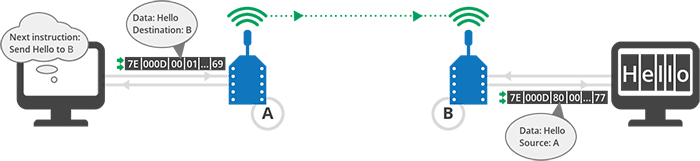
\includegraphics[scale=.7]{api_mode.png}
\caption{ارتباط سریال در حالت \lr{API} \cite{Digi}}\label{fig:api_mode}
\end{figure}


\section{پایگاه داده‌ی سری زمانی}

سری زمانی یک توالی مرتب‌شده از مقادیر یک متغیر در فواصل زمانی مساوی است. بنابراین سری زمانی یک توالی از داده‌های زمان گسسته است\cite{naqvi2017time}. داده‌های لرزش جمع‌آوری‌شده در این پروژه نیز از نوع سری زمانی هستند. جهت ذخیره‌سازی، پردازش و مدیریت بهینه این داده‌ها نیاز به یک پایگاه داده داریم.


\lr{InfluxDB} یک پایگاه داده سری زمانی بدون طرحواره\LTRfootnote{Schemaless} منبع باز با اجزای اختیاری منبع بسته است که توسط \lr{InfluxData} توسعه یافته است. این به زبان برنامه‌نویسی گو\LTRfootnote{Go} نوشته شده‌است و برای مدیریت داده‌های سری زمانی بهینه شده‌است. این یک زبان پرس و جو\LTRfootnote{Query Language} مانند \lr{SQL} را ارائه می دهد. نسخه منبع باز که در \cref{fig:influx} \cite{influx} نشان داده شده‌است، یک پلتفرم پایگاه داده سری زمانی کامل را با خدمات مختلف از جمله هسته \lr{InfluxDB} فراهم می‌کند و می‌تواند بر روی ابر و در محل روی یک گره واحد اجرا شود.

\begin{figure}[!h]
\centering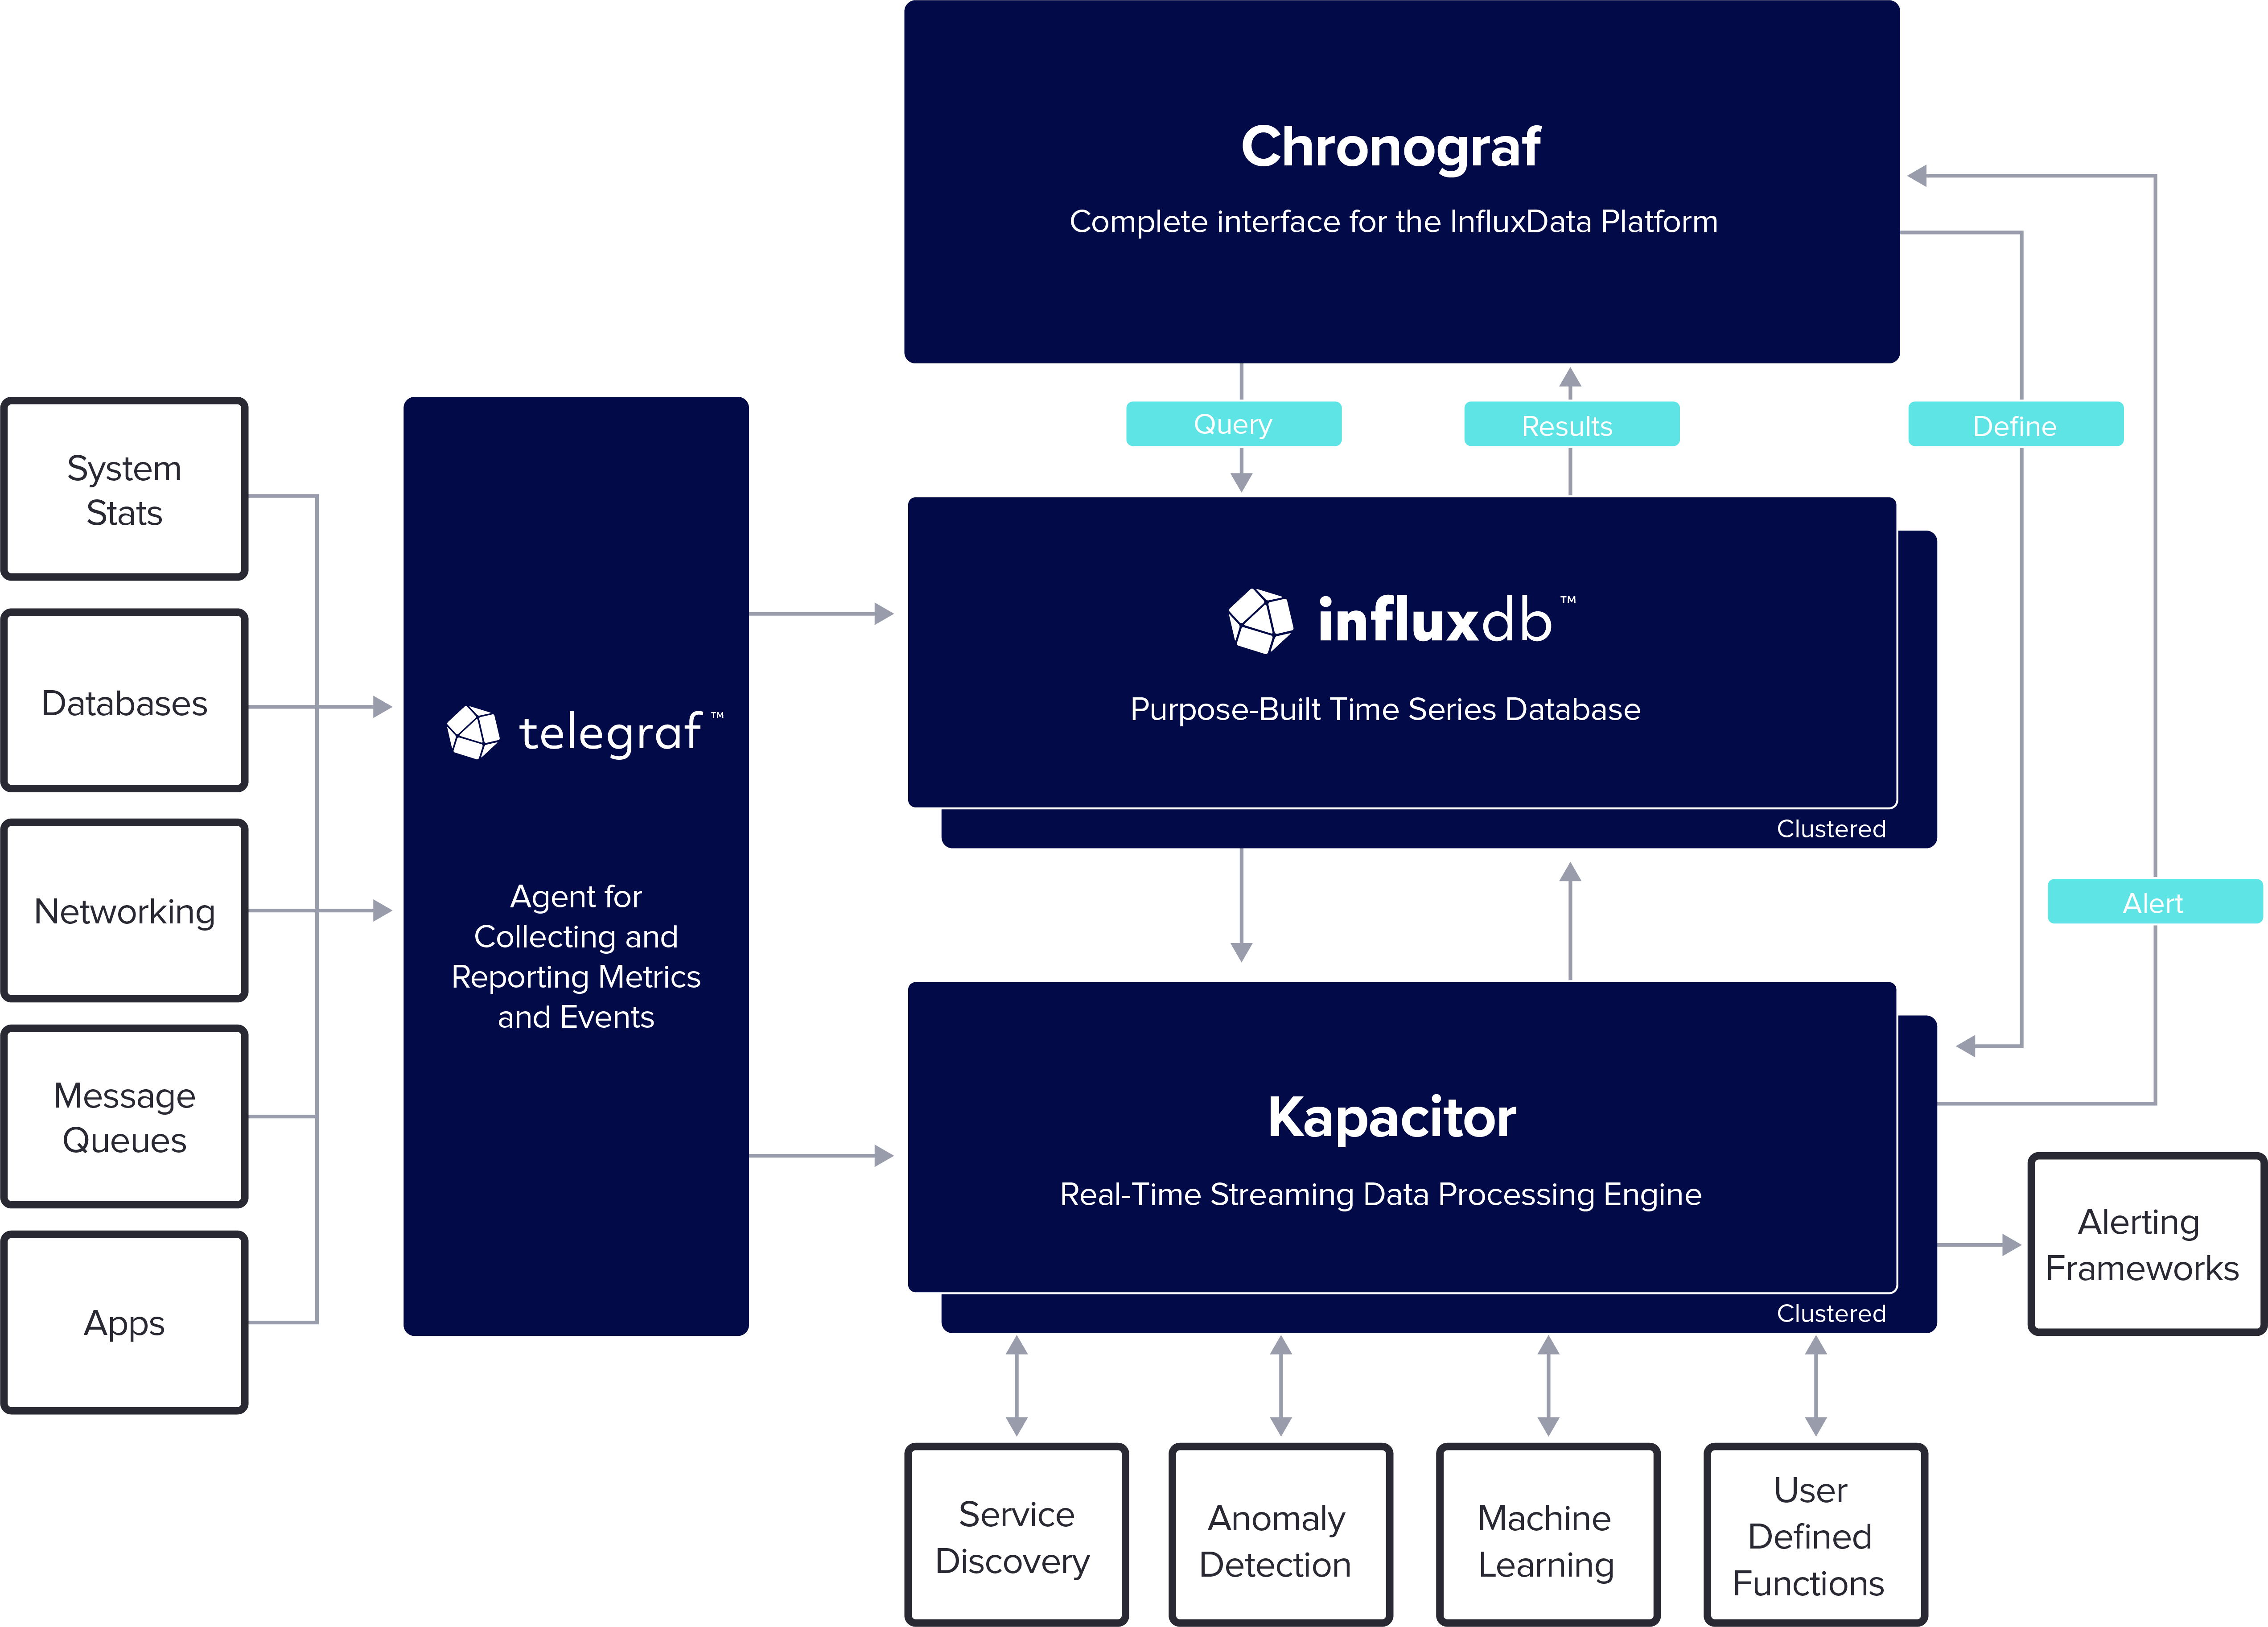
\includegraphics[scale=.11]{influx.png}
\caption{پلتفرم متن باز پایگاه داده سری زمانی \lr{InfluxDB} \cite{influx}}\label{fig:influx}
\end{figure}

استفاده از پایگاه داده \lr{InfluxDB} برتری‌هایی نسبت به سایر پایگاه داده‌ها دازد که باعث شد ما از آن برای ذخیره داده‌های لرزش استفاده کنیم. این برتری‌ها عبارتند از:

\begin{itemize}
\item طراحی اختصاصی برای داده‌های سری زمانی و عملکرد بهینه در خواندن و نوشتن این داده‌ها.
\item افزودنی‌های رایگان و متعدد مانند \lr{HTTP API} که باعث تسریع و راحتی توسعه می‌شود.
\item پشتیبانی از تعداد بالای زبان‌های برنامه‌نویسی.
\item پشتیبانی از زبان پرس و جویی مانند \lr{SQL} بنام \lr{InfluxQL} که یادگیری و پیاده‌سازی را راحت‌تر می‌کند.
\end{itemize}

